\documentclass{standalone}
\usepackage{tikz}
\usetikzlibrary{arrows}
\begin{document}
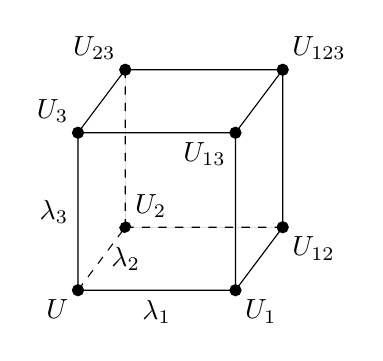
\begin{tikzpicture}[scale=1]

\draw[fill=black]
(2,0) circle(2pt) node[below right] {$U_1$} --
(2,2) circle(2pt) node[below left] {$U_{13}$} --
(0,2) circle(2pt) node[above left] {$U_3$} --
(0,0) circle(2pt) node[below left] {$U$} -- (2,0);

\begin{scope}[xshift=6mm,yshift=8mm]
\draw[fill=black]
(2,0) circle(2pt) node[below right] {$U_{12}$} --
(2,2) circle(2pt) node[above right] {$U_{123}$} --
(0,2) circle(2pt) node[above left] {$U_{23}$};
\draw[fill=black,dashed]
(0,2) -- (0,0) circle(2pt) node[above right] {$U_2$} -- (2,0);
\end{scope}

\draw[dashed] (0,0) -- (.6,.8);
\draw (2,0) -- (2.6,.8);
\draw (0,2) -- (.6,2.8);
\draw (2,2) -- (2.6,2.8);

\node[below] at (1,0) {$\lambda_1$} ;
\node[right] at (.3,.4) {$\lambda_2$} ;
\node[left] at (0,1) {$\lambda_3$} ;
%
%\fill[red] (0,0) circle(2pt);
%\fill[red] (2,0) circle(2pt);
%\fill[red] (0,2) circle(2pt);
%\fill[red] (.6,.8) circle(2pt);
%\fill[blue] (.6,2.8) circle(2pt);
%\fill[blue] (2,2) circle(2pt);
%\fill[blue] (2.6,.8) circle(2pt);

\end{tikzpicture}
\end{document}